\newgeometry{left=5cm, right=4cm,bottom=4cm, top=4cm}
\chapter{Reconstruction of Physics Object}\label{chap:obj} \vspace{1cm}

The raw ATLAS  data, containing  detectors signals of all  read-out channels, need to
 undergo  several reconstruction steps before they can be analyzed. Reconstruction software is developed 
 within the object oriented ATLAS reconstruction software framework ATHENA~\cite{Athena}, which allow for reconstruction and 
identification of various objects corresponding to physics particles traversing the detector.


This chapter briefly describes the ATLAS reconstruction strategies for physics objects relevant for the 
analysis of the neutal MSSM $A/h/H \rightarrow \tautau$ decay channel presented in this thesis.
For a detailed overview of the ATLAS detector reconstruction software  see~\cite{AtlasCSCBook}. 

\restoregeometry
\clearpage

\section{Reconstruction of Charged Particle Tracks}
The reconstruction of charged particles tracks and interaction vertices is based on the measurements in the inner detector,
which allow for the reconstruction of tracks within the pseudorapidity range of $|\eta| < 2.5$. 
A track is characterized by its four-momentum vector and two impact parameters: $d_0$, i.e.,  the distance 
of closest approach between the track and the interaction point in the transverse plane and $z_0$, i.e.
the $z$ coordinate of the track calculated at the same point. 

Tracks are reconstructed  by the Inner Detector track reconstruction software~\cite{IDtracking}.
First raw data from the pixel and SCT detectors are transformed in three dimensional space points 
which are called ``hits'', while the  TRT detector information is translated into drift circles. 
Then, track seeds are formed from a combination of space-points in the three pixel layers and the first SCT layer, these
seeds are then extended throughout the SCT to form track candidates. The tracks candidate are fitted 
using a \emph{Kalman filter} algorithm~\cite{Kalman}, ambiguities in the cluster-to-track association are resolved
and fake tracks are rejected. The selected tracks are then extended to the TRT and finally refitted with the full information of all three
detectors. To help improve tracking efficiency for secondary tracks coming from photon conversion or decays of long-lived 
particles (like kaons), a complementary algorithm searches for unused track segments in the TRT, which will be then extended
towards the SCT and the pixel in a very similar way as described for the default algorithm.
All tracks found with $\pt > 100$ MeV are written to the database.


\section{Vertex Reconstruction}
The vertex reconstruction algorithm and its performance are described in full detail in~\cite{AtlasCSCBook,VertexPerf} and
only briefly summarized here.
%say good tracks
The vertex finding is performed as follows:  a set of well reconstructed tracks are selected,
a vertex is seeded according to the global maximum of the selected tracks $z$ coordinate distribution, the tracks $z$ coordinate 
is computed with respect the expected average collision point. 
An \emph{adaptive vertex fitting} algorithm~\cite{Vertex} determines the vertex position taking as input the vertex seed position and the 
tracks around it. Tracks that are incompatible with the found vertex by more than seven standard deviation
are used to seed the next vertex. The iteration continues until no tracks are left or no additional vertex can be found.
The procedure depends  on the expected position of the average interaction point, which is monitored 
during LHC data taking and is computed every few minutes with the method described in~\cite{beamspot}.

The vertex with the larger sum of tracks $\pt$ associated is identified as the \emph{primary vertex} (PV), 
which is the interaction point related to the hard scattering of the event. All the other vertices are assumed to result from
minimum bias interaction and are called \emph{pile-up} vertices.
In data recorded during 2012, an average of 21 multiple interaction are occurred per bunch crossing,
such a high vertex multiplicity strongly affects the ambient energy density in the event, 
a correct pile-up description is then crucial for MC simulation. In ATLAS, simulated events are produced under
various pile-up conditions, the events are then weighted according to the average interaction
per bunch crossing recorded in data.


\section{Electrons Reconstruction} \label{sec:elec}
Electron are reconstructed combining EM calorimeter and Inner Detector information,
the ATLAS dedicated electron reconstruction algorithm is presented in~\cite{electronAlgo}.
The electron reconstruction starts from clusters of EM calorimeter cells, 
tracks are sought in the Inner Detector to match the clusters, special care is taken in order to account for 
Bremsstrahlung losses during the track matching stage. 
An electron candidate is defined as a cluster in the EM calorimeter combined with a track.
%Once an electromagnetic shower in the calorimeter is 
%found to match with one or more tracks, the combination of those is considered as an electron candidate.  
The electron energy is computed as 
a weighted average between the cluster energy and the track momentum, several corrections are applied to
take into account energy loss in the material of the Inner Detector and effect of electromagnetic shower 
leakage. The electron direction is taken from the corresponding track parameters. 

Further selection are applied to the electron candidates to reduce contamination
from photon conversion and hadronic jet, three different identification criteria are provided:
\begin{itemize}
	\item Loose: selections related to the shape of the shower and to hadronic leakage are applied.
	\item Medium: additionally to the loose requirements, information on the strip layer of the electromagnetic
	calorimeter is used, stricter track matching requirements are also applied.
	\item Tight: additionally to medium requirements, 
		converted photons are rejected by requiring a hit in the Inner Detector b-layer (if the module
		is expected to be operating), TRT electron identification capability is employed.
\end{itemize}

The electron identification performances are compared between data and simulation in~\cite{eleEff}, 
correction to the electron identification efficiency are estimated and 
applied as weight to simulated electron candidates. Additional corrections are applied to the energy scale and resolution
of simulated electron to match the one in data according to~\cite{eleEnergy}.
Finally, the electrons used in the presented analysis are rejected if matching 
with a region of the calorimeter with readout problems or suffering from high noise.

Prompt electrons, coming from the decay of a resonance like the $Z^0$ boson or the Higgs boson are very
likely to be \emph{isolated}, i.e. very little activity is expected in their surroundings, this is in contrast
to electron that come from decay of hadrons, which instead will be likely to be embedded in a jet of particle.
Two isolation variables are then defined by the sum of the energy in a $\Delta R = \sqrt{\Delta\phi^2 + \Delta\eta^2}$ 
cone around the electron candidate:
\begin{itemize}
	\item Track isolation $\pt^{cone}$: which is the scalar sum of the track $\pt$ in a $\Delta R \leq 0.4$
	cone around the electron, the electron track is not considered.
	
	\item Calorimeter isolation $E_T^{cone}$: which is the scalar sum of  topological cluster transverse energy
	 in a  $\Delta R \leq 0.2$ cone around the electron. Cluster associated to the electron are not considered.
	 This variable is corrected as a function of the vertex multiplicity in the event in order to assure a constant 
	 selection efficiency.
\end{itemize}



\section{Muons Reconstruction}\label{sec:muon}
ATLAS employs a variety of strategies for identifying and reconstructing muons, 
the main detector used for this purpose is the Muon Spectrometer, which may be supplemented with
others detectors informations. A detailed description
of the muon reconstruction algorithms and their performance is reported in~\cite{AtlasCSCBook},
in the following only the muon reconstruction strategy relevant for this thesis is described.

The STACO \emph{combined} muon algorithm~\cite{staco} associate tracks found in the
Muon Spectrometer with the corresponding Inner Detector track and calorimeter information, the muons are then
 identified at their production vertex with optimum parameter resolution.
First  track segment are reconstructed in each of the three
muon station, segments are then liked together to form a track. The muon track is
extrapolated to the Inner Detector taking into account energy loss and multiple scattering in the calorimeters,
then, it is  matched with a Inner Detector track via $\chi^2$ matching. Finally
a statistical combination of the Inner Detector and Muon Spectrometer tracks is performed to obtain a combined vector. 

Muon reconstruction efficiency, momentum scale and resolution are evaluated in~\cite{muoneffres},
performance are compared with MC simulation and a set of corrections, aimed to restore agreement
between data and simulation, are provided. Correction on muon momentum scale, resolution and reconstruction
efficiency are applied to muons in the presented analysis.

Isolation variable, as described for electrons, are also implemented for muons, the only exception 
is the use of calorimeter cluster with fixed size (towers) in the definition of $E_T^{cone}$.
Similar pile-up corrections are also used for muons.  



\section{Jets Reconstruction and Energy Calibration}
Jets are reconstructed in ATLAS by means of the FastJet package~\cite{fastjet}, 
which provides a broad range of jet finding algorithms and analysis tools. 
In the following jet reconstruction methods relevant for the
analysis presented in this theses are briefly described, for more detail see~\cite{AtlasCSCBook}.

In general, jets may be reconstructed out of any set of four vector objects, 
however in ATLAS, the most important detectors for jet reconstruction are the ATLAS calorimeters.
Calorimeter cells are grouped together by a clustering algorithm forming what are called \emph{topological clusters}~\cite{TopoClusterAlgo},
those are three-dimensional cluster representing the energy deposition of the shower.
the clustering starts with seed cells with a signal-to-noise ratio greater that a certain threshold, 
all nearby cells are grouped to the seed cells if they passes a second, lower, signal-to-noise ratio threshold.

Topological clusters are then fed to an \emph{anti-$k_t$} algorithm~\cite{antikt}. The algorithm defines a metric
to assess distances between the clusters $i$ and $j$, the metric is defined as follows:
\begin{align}
d_{ij} &= \text{min}(\frac{1}{k_{t,i}^2}, \frac{1}{k_{t,j}^2}) \cdot \frac{\Delta R_{ij}^2}{R^2}  \\
d_i   &= \frac{1}{k_{t,i}^2} 
\end{align}
where $k_{t,i}$ is the $\pt$ of the cluster $i$ and $\Delta R_{ij}^2 = \sqrt{\Delta\phi_{ij}^2 + \Delta\eta_{ij}^2}$. For
the presented  analysis $R=0.4$ is chosen.
If the distance between two cluster $d_{ij}$ is smaller that $d_i$ the clusters are grouped together and their four momentum
summed, otherwise their are kept as single entity. The clustering procedure is iterated until no cluster can be further merged. 
The metric is designed in a way that high $\pt$ clusters will accumulate the soft activity surrounding them leading to conical
jet shapes. 

Given the high pile-up environment of LHC  is important to distinguish jets coming from the hard scattering process and those
related to pile-up interaction, for this purpose, a technique called \emph{jet vertex fraction} (JVF) is implemented in the 
ATLAS jet reconstruction software.
The JVF relies on Inner Detector informations, it is defined as the $\pt$ weighted fraction of tracks pointing
to to the primary vertex associated to the jet:
\begin{equation}
\text{JVF} = \frac{\sum\limits_{PV-tracks}\pt}{\sum\limits_{tracks}\pt}
\end{equation} 
the jet vertex fraction  is only available within Inner Detector coverage $|\eta| < 2.5$,
while calorimeter jet reconstruction is possible up to $|\eta| < 4.5$.

\paragraph{Calorimeter Jet Energy Calibration}
The ATLAS calorimeters were calibrated using test beam electrons~\cite{EMcalibration}, however  the response
to electromagnetic shower  is different from the one to hadronic shower. A dedicated jet energy scale
(JES) calibration is then performed by means of MC simulation~\cite{jesinsitu}: 
jet energy is corrected to correspond, as a mean value, to the simulated energy 
of the hadronizing parton origin of the jet. The direction of the jet is also corrected to constraint it to point
to the primary vertex instead to the center of the ATLAS detector. A set of corrections are then evaluated to take into account
effect of pile-up~\cite{jespileup, jesarea}. Jet resolution is also corrected in MC to better describe the data~\cite{jer}. 
Finally, several jet energy scale correction are applied for a better agreement between 
data and simulation, those corrections are evaluated based on 2011 ATLAS data and  
exploits several techniques, JES systematic uncertainty due not perfect MC modeling are also evaluated,
a full description of JES "in-situ" methodology corrections and related systematics uncertainties are 
described in~\cite{jesinsitu, JES}. %all the correction are combined together obtaining the final JES


\section{Jet b-Tagging}
The typical decay length of b-hadron at ATLAS is of the order of few millimeter. Exploiting the high precision of the
Inner Detector tracker is possible to identify jet originating from b-quarks with respect to other flavors, 
those jets are called \emph{b-jets} and the identification technique used \emph{b-tagging}.

Several algorithm has been developed in ATLAS for jet b-tagging, the relevant b-tagging algorithm
to this thesis are briefly described in what follows, for more detailed description see~\cite{AtlasCSCBook}.
The first step of jet b-tagging is to associate tracks to jets based on a $\Delta R$ cone matching, those tracks 
should satisfy strict selection criteria aimed to assure good quality 
and to reject tracks likely to come from strange hadron decays or photon conversion. 
For the discrimination between b-jet and light-jet (and in some cases also c-jet) 
algorithms uses the MC prediction of the distribution of some discriminating variable 
for the two hypothesis.
Given the relatively high mass of b-hadrons, the tracks
associated with b-jet will have spreaded impact parameters, this feature is used by the IP3D b-jet tagging 
algorithm, where a discriminating variable is implemented based on the impact parameter significances of the tracks
associated to the jet. An alternative approach, used by the $SV1$ algorithm, is instead  to searches for inclusive 
secondary vertex formed by the decay products of the b-hadron,  the search includes also 
the subsequent charm hadron decays. Another algorithm, called JetFitter~\cite{jetfitter}, uses instead the direction of the jet
to fully reconstruct the decay chain of b-hadron, the assumption made is that the decayed particles will lie along the
jet axis. Finally, the three algorithm just described are combined together using an
artificial neural network to maximize the discriminating power, the output of this neural network is referred
as $MV1$ and is used in the search presented in this thesis. 

\begin{figure}[tp]
     \begin{center}

            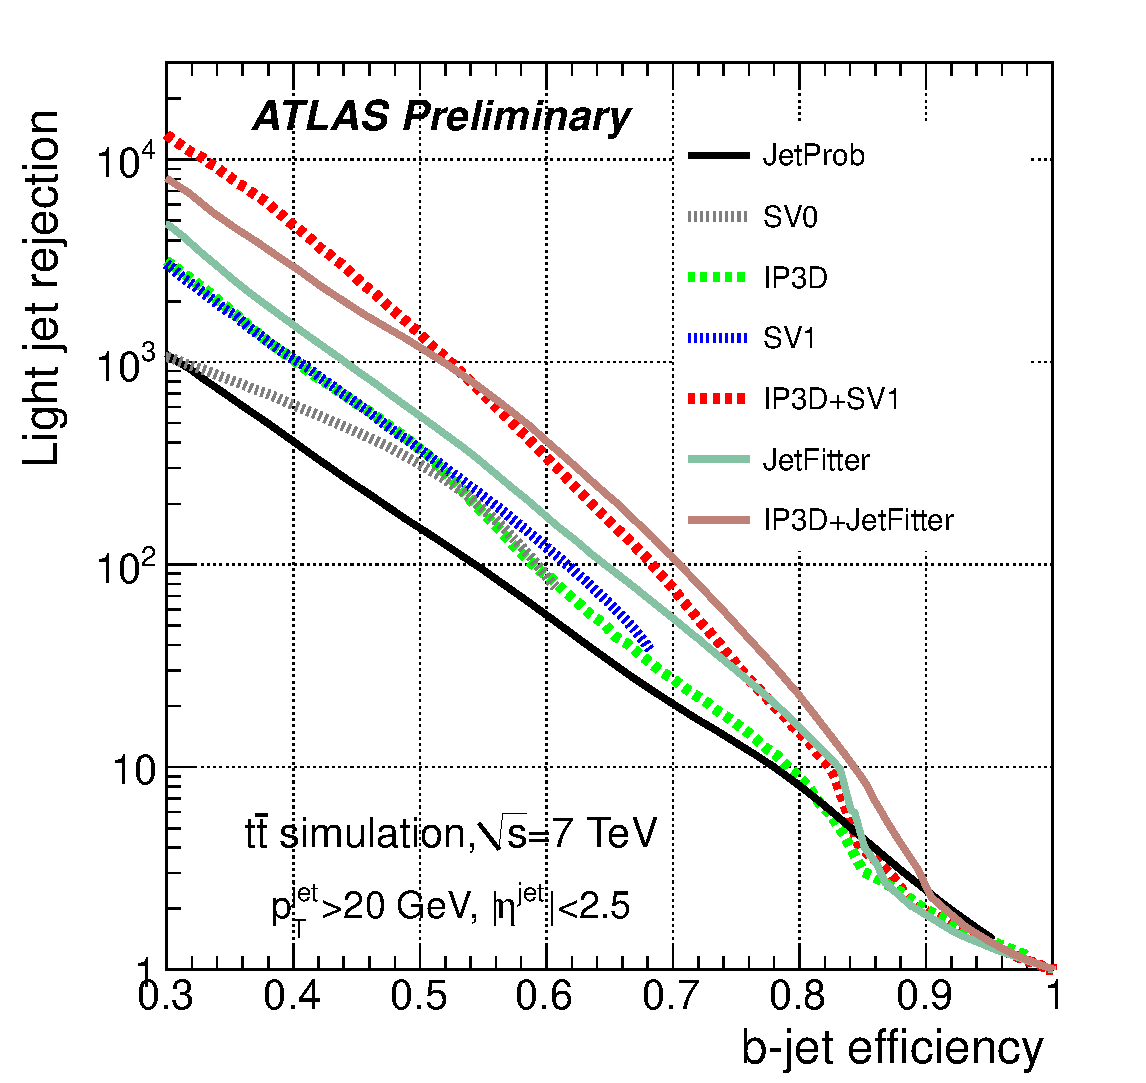
\includegraphics[width=0.6\textwidth]{figure/obj/btag_perf.pdf}

    \end{center}
    \caption{Light-jet rejection as a function of the b-jet tagging efficiency for different tagging algorithms~\cite{btagPerf}.
	    Rejection here is defined as the inverse of mistagging rate, and the distributions are referred to a 
		$\ttbar$ sample.}
   \label{fig:beff}
\end{figure}

The performance of the mentioned algorithms are evaluated in data  and compared to simulation in~\cite{btagPerf}.
B-hadron tagging efficiency and mistagging rate are the most common feature that describes the performance of a
b-tagging algorithm, Figure~\ref{fig:beff} shows the b-tagging efficiency as a function of the inverse of the mistagging rate
for different b-tagging algorithm, the tagging efficiency $\epsilon_b^{\ttbar}$ is usually referred to b-hadron in $\ttbar$ events
and totally specify a b-tagging selection point.
Correction due to non perfect modeling of b-tagging performance are evaluated by means of several methods
for 2012 data in~\cite{BtaggingScaleFactors, BtaggingScaleFactorsNew} and used as event weights in MC simulation.




\section{Missing Transverse Energy } \label{sec:met}
The missing transverse energy, \met, is the absolute value of the vectorial sum of the transverse momenta
in the event. Undetected particles, such as neutrinos leads to an unbalance of the total
transverse momentum, thus, to a non zero \met.

Reconstruction and calibration of \met at ATLAS is described in detail in~\cite{ETMISS}. 
The missing transverse energy relies on the reconstruction of all physics object 
in the event: it includes muons and their energy deposit in the calorimeter, electron, jets (weighted by their JVF), 
Inner Detector tracks (to take into account low-$\pt$ particles not well reconstructed in the calorimeters),
photons and $\tau$ leptons. The calorimeters cells are then calibrated depending on the
object they are associated with. Cells not associated to any object are included in the so called
 ``CellOut term'', this term,  together with the one related to jets with $10 < \pt < 20$ GeV
are referred to as the \emph{soft term} of the missing transverse energy.
The soft term is found to be very sensitive to pile-up, a solution to reduce this effect 
is to scale it by its soft-term-vertex-fraction (STVF), which is calculated exactly as for JVF in jets.

A description of the performance of the ATLAS \met reconstruction and calibration may be found in~\cite{ETMISS2}.


\section{Tau Hadronic Decay}\label{sec:tau}
The reconstruction of hadronically decaying $\tau$ candidates (in the following $\tau_h$)
is described in detail in~\cite{AtlasCSCBook}.
A $\tau_h$ candidate is seeded by reconstructed calorimeter jets with $\pt > 10$ GeV and $|\eta| < 2.5$,
tracks are then associated to the jet and a combination between tracking and calorimeters informations
is performed.  Hadronic tau decays can be distinguished from jets by their low track multiplicity and 
narrow clustering of electromagnetic and hadronic calorimeter activity. The $\tau_h$ identification 
in ATLAS is performed by a multivariate discriminant based on Boosted Decision Trees (BDTs)~\cite{ATLASTAUIDnew}.
One BDT discriminant has been developed to discriminate $\tau_h$  from quark and gluon 
initiated jets and a separate BDT was developed to reject electrons.
The analysis presented in the next chapter requires one or three charged tracks associated to the $\tau_h$ candidate, 
for the identification a ``Medium'' BDT working point is chosen, additionally, a BDT-based electron veto is 
applied.

\section{Overlap Removal} \label{sec:olr}
Reconstruction of the physics object defined in the previous section may sometimes
be ambiguous, for example, an hadronic $\tau$ is always reconstructed also as a jet.
To avoid double counting of the same physics object a procedure of overlap removal is performed
in the presented analysis. Physics object of different sort are matched in a cone of $\Delta R <0.2$,
if matching occurs, the object with the lowest ranking is removed from the event. 
Physics object are ranked according to the following order: first muon, then electron, hadronic $\tau$ 
and finally jets.

\section{Trigger}
The ATLAS trigger system~\cite{trigger} consists of three stages. The Level-1 (L1) trigger is a
hardware trigger which reduces the event rate to approximatively 100 kHz and selects the Regions of
Interest (RoI) to be further investigated by the High Level Trigger (HLT). The HLT
comprises the Level-2 (L2) trigger employing fast reconstruction algorithms and the
Event Filter (EF) exploiting the full ATLAS event reconstruction.

In the presented search two triggers are employed: an electron EF trigger, which selects data presenting 
an electron with $\pt >24 $~GeV and a combined muon-electron EF trigger, which requires a muon with $\pt > 8$ GeV and 
an electron with $\pt > 12$~GeV. Detailed description of the muon and electron triggers can be found in~\cite{triggermu,triggere}.
Trigger efficiency for both triggers is evaluated and compared with MC prediction, corrections as function of lepton
direction and momentum are derived to match MC trigger efficiency to data~\cite{triggermu,triggere}, 
those corrections are applied in the presented analysis.

\section{Truth Particles}
In case of a simulated event, the ATLAS reconstruction software provides information regarding
simulated particles (also called \emph{truth-particles}), their identity, properties, decays and 
interactions are stored in the event  based on the conventions defined in~\cite{hepmc}.
A particle is defined stable if $c \tau > 1$~m, where $\tau$ is its mean life time, particle emerging from 
interaction with the detector are excluded from this definition. 
Each particle has an associated ``barcode'' which is a unique identifier for that particle
in that event. Jets reconstructed from stable particles are called \emph{truth-jets}.

